\documentclass[aspectratio=43,11pt]{beamer}
\usepackage{fontspec}
\usepackage{pgfplots}\pgfplotsset{compat=1.18}
\usepackage{tikz}\usetikzlibrary{positioning}
\usecolortheme{default}
\setbeamertemplate{navigation symbols}{}
\definecolor{teal0}{RGB}{0,128,128}
\definecolor{burnt}{RGB}{204,85,0}
\definecolor{ink}{RGB}{33,37,41}
\definecolor{paper}{RGB}{250,249,246}
\setbeamercolor{background canvas}{bg=paper}
\setbeamercolor{frametitle}{fg=teal0}
\setbeamercolor{title}{fg=teal0}
\setbeamercolor{structure}{fg=burnt}
\setbeamercolor{normal text}{fg=ink}
\setbeamerfont{frametitle}{series=\bfseries}
\setbeamertemplate{frametitle}{\vskip6pt\usebeamerfont{frametitle}\usebeamercolor[fg]{frametitle}\insertframetitle\par\vskip-2pt{\color{burnt}\rule{\linewidth}{1.2pt}}}
\setbeamertemplate{itemize item}{\color{burnt}\textbullet}
\setbeamertemplate{itemize subitem}{\color{teal0}--}
\newcommand{\foot}[1]{\vfill{\scriptsize\color{teal0}#1}}
\pgfplotsset{
  every axis/.append style={font=\small, axis line style={gray!50}, tick style={gray!50},
    grid=major, major grid style={gray!20}, label style={color=ink}, tick label style={color=ink}},
  A/.style={fill=teal0,draw=teal0!70}, C/.style={fill=burnt,draw=burnt!70},
}

\title{\textbf{Grounding LLMs in a Formal Ontology}}
\subtitle{A pervasive knowledge-graph binding that makes every model measurably smarter}
\author{\textbf{VisionFlow} \textbullet\ VisionClaw \textbullet\ Agentbox}
\date{\textcolor{burnt}{\url{http://www.visionflow.info}} \quad\textbullet\quad 2026-06-14}

\begin{document}

{\setbeamertemplate{footline}{}
\begin{frame}[plain]
  \vfill\centering
  {\color{teal0}\Huge\textbf{Grounding LLMs in a\\[2pt] Formal Ontology}\par}
  \vskip10pt
  {\large A pervasive knowledge-graph binding that makes\\ \emph{every} model measurably smarter\par}
  \vskip16pt
  {\color{burnt}\Large\textbf{F1 0.37 \;$\rightarrow$\; 0.81}}\;{\normalsize across 5 LLMs}\par
  \vskip20pt
  {\large\textbf{VisionFlow} \;\textbullet\; VisionClaw \;\textbullet\; Agentbox\par}
  \vskip6pt
  {\color{burnt}\large\url{http://www.visionflow.info}\par}
  \vfill
\end{frame}}

\begin{frame}{The headline}
  \begin{center}
  \vskip4pt
  {\Large Connecting a \textbf{formal ontology} (4{,}196 OWL classes, 222k inferred axioms)\\ to \emph{every} AI call lifts factual recall \textbf{across the board}.}
  \vskip14pt
  
\begin{tikzpicture}
  \node[draw=teal0,line width=1.2pt,rounded corners,inner sep=10pt] {\color{teal0}\Huge\textbf{+0.44 mean F1}};
  \end{tikzpicture}
  \vskip10pt
  {\large Augmented \textbf{0.81} vs.\ ungrounded \textbf{0.37} \quad\textbullet\quad hallucination roughly \textbf{halved}}\\[2pt]
  {\normalsize 5 models \;\textbullet\; 16 KG-grounded questions \;\textbullet\; 160 isolated runs \;\textbullet\; objective scoring}
  \end{center}
  \foot{Lead, not buried: the binding works, and it is model-agnostic.}
\end{frame}

\begin{frame}{What we built}
  \begin{itemize}
    \item \textbf{VisionFlow} --- the immersive 3D knowledge-graph + agent platform (\url{visionflow.info}).
    \item \textbf{VisionClaw} --- the Rust engine: Oxigraph/Whelk ontology store, GPU physics, real-time graph.
    \item \textbf{Agentbox} --- the sovereign agent runtime; 100+ skills, MCP tooling, governed memory.
  \end{itemize}
  \vskip6pt
  {\color{teal0}\textbf{The final piece:}} a \emph{pervasive ontology binding} so any AI call can ground itself in the
  formal knowledge graph --- read-pervasive, write-governed, budget-bounded, fail-open.
  \foot{Features are legion; this deck leads with the one that ties them together.}
\end{frame}

\begin{frame}{The binding, in one picture}
  \centering
  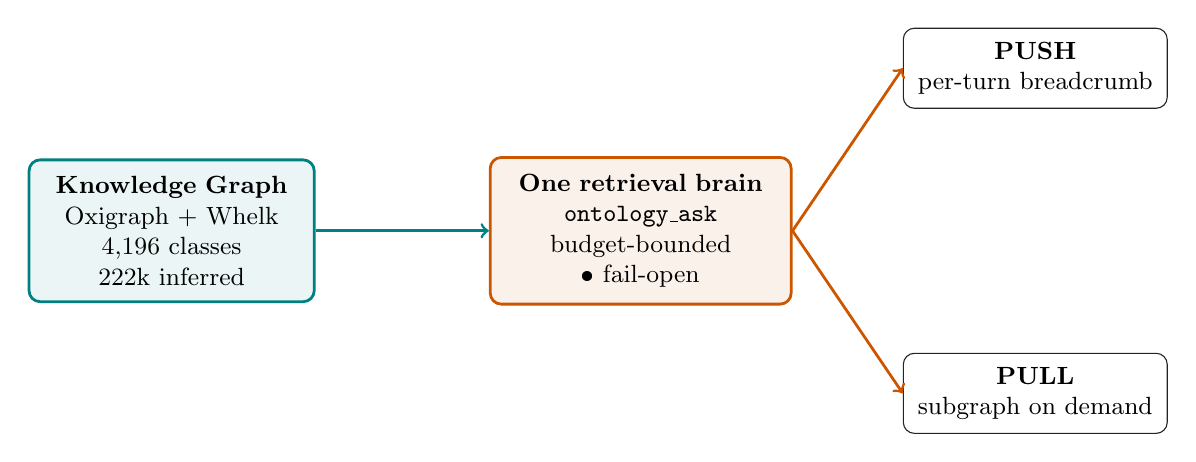
\begin{tikzpicture}[node distance=7mm,every node/.style={font=\small}]
    \node[draw=teal0,line width=1pt,rounded corners,fill=teal0!8,inner sep=6pt,text width=3.2cm,align=center] (kg) {\textbf{Knowledge Graph}\\Oxigraph + Whelk\\4{,}196 classes\\222k inferred};
    \node[draw=burnt,line width=1pt,rounded corners,fill=burnt!8,inner sep=6pt,text width=3.4cm,align=center,right=22mm of kg] (brain) {\textbf{One retrieval brain}\\\texttt{ontology\_ask}\\budget-bounded \textbullet\ fail-open};
    \node[draw=ink,rounded corners,inner sep=5pt,text width=3.0cm,align=center,above right=6mm and 14mm of brain] (push) {\textbf{PUSH}\\per-turn breadcrumb};
    \node[draw=ink,rounded corners,inner sep=5pt,text width=3.0cm,align=center,below right=6mm and 14mm of brain] (pull) {\textbf{PULL}\\subgraph on demand};
    \draw[->,teal0,line width=1pt] (kg)--(brain);
    \draw[->,burnt,line width=1pt] (brain.east)--(push.west);
    \draw[->,burnt,line width=1pt] (brain.east)--(pull.west);
  \end{tikzpicture}
  \vskip8pt
  \begin{itemize}\small
    \item \textbf{Read-pervasive:} every agent, consultant and turn can consult the KG.
    \item \textbf{Write-governed:} proposals are auth-gated and queued; derived facts are fenced.
  \end{itemize}
  \foot{One shared library --- the MCP tool, the consultant seam and the CLI share identical grounding.}
\end{frame}

\begin{frame}{How we measured it (objectively)}
  \begin{itemize}
    \item \textbf{KG-as-oracle:} ground truth generated \emph{from the graph itself} --- neighbours, subclasses,
          class existence --- so scoring is deterministic, not subjective.
    \item \textbf{Clean A/B:} each cell is an \emph{isolated} session given only the question;
          augmented arm receives the ontology subgraph, control uses parametric knowledge only.
    \item \textbf{5 models $\times$ 16 questions $\times$ 2 conditions} = \textbf{160 isolated runs}.
    \item \textbf{Grader:} precision / recall / F1 + hallucination, token-set matched.
  \end{itemize}
  \foot{Anthropic Opus/Sonnet/Haiku, Google Gemini 2.5 Pro, Z.AI GLM-5.2.}
\end{frame}

\begin{frame}{Result: every model wins}
  \centering
  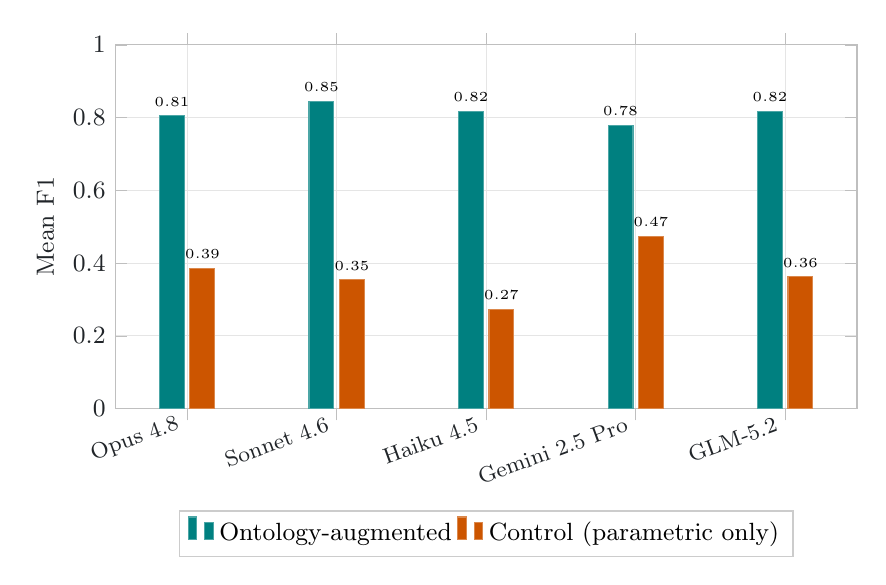
\begin{tikzpicture}
  \begin{axis}[ybar,width=11cm,height=6.2cm,bar width=9pt,ymin=0,ymax=1,ylabel={Mean F1},
    symbolic x coords={Opus 4.8,Sonnet 4.6,Haiku 4.5,Gemini 2.5 Pro,GLM-5.2},xtick=data,x tick label style={rotate=20,anchor=east,font=\footnotesize},
    enlarge x limits=0.12,legend style={at={(0.5,-0.28)},anchor=north,legend columns=2,draw=gray!40},
    nodes near coords,nodes near coords style={font=\tiny}]
  \addplot[A] coordinates {(Opus 4.8,0.805) (Sonnet 4.6,0.845) (Haiku 4.5,0.817) (Gemini 2.5 Pro,0.778) (GLM-5.2,0.817)};
  \addplot[C] coordinates {(Opus 4.8,0.385) (Sonnet 4.6,0.354) (Haiku 4.5,0.273) (Gemini 2.5 Pro,0.473) (GLM-5.2,0.362)};
  \legend{Ontology-augmented,Control (parametric only)}
  \end{axis}\end{tikzpicture}
  \foot{Universal lift: +0.31 to +0.54 F1. The smallest model (Haiku) gains the most.}
\end{frame}

\begin{frame}{Result: hallucination roughly halved}
  \centering
  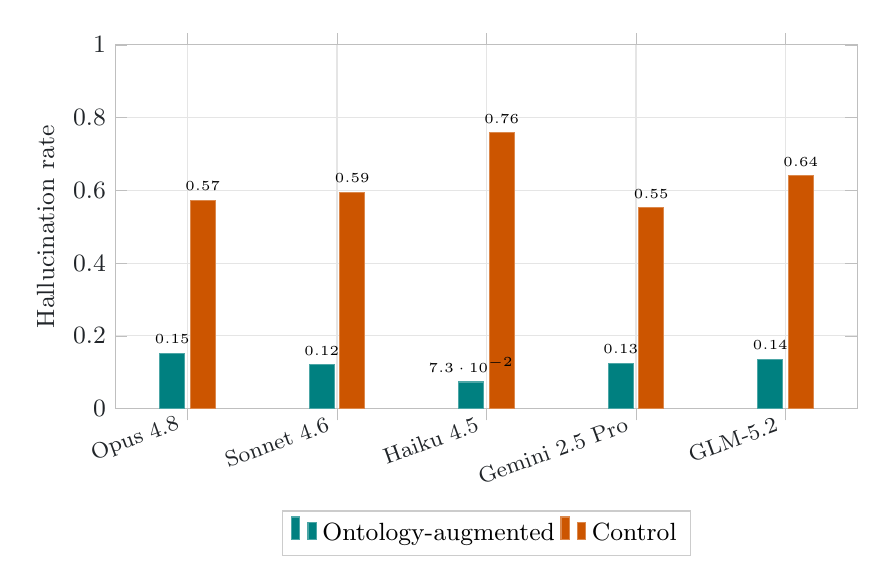
\begin{tikzpicture}
  \begin{axis}[ybar,width=11cm,height=6.2cm,bar width=9pt,ymin=0,ymax=1,ylabel={Hallucination rate},
    symbolic x coords={Opus 4.8,Sonnet 4.6,Haiku 4.5,Gemini 2.5 Pro,GLM-5.2},xtick=data,x tick label style={rotate=20,anchor=east,font=\footnotesize},
    enlarge x limits=0.12,legend style={at={(0.5,-0.28)},anchor=north,legend columns=2,draw=gray!40},
    nodes near coords,nodes near coords style={font=\tiny}]
  \addplot[A] coordinates {(Opus 4.8,0.151) (Sonnet 4.6,0.12) (Haiku 4.5,0.073) (Gemini 2.5 Pro,0.125) (GLM-5.2,0.135)};
  \addplot[C] coordinates {(Opus 4.8,0.573) (Sonnet 4.6,0.594) (Haiku 4.5,0.758) (Gemini 2.5 Pro,0.552) (GLM-5.2,0.64)};
  \legend{Ontology-augmented,Control}
  \end{axis}\end{tikzpicture}
  \foot{Grounding replaces plausible-but-wrong guesses with the graph's actual vocabulary.}
\end{frame}

\begin{frame}{Where grounding helps most}
  \centering
  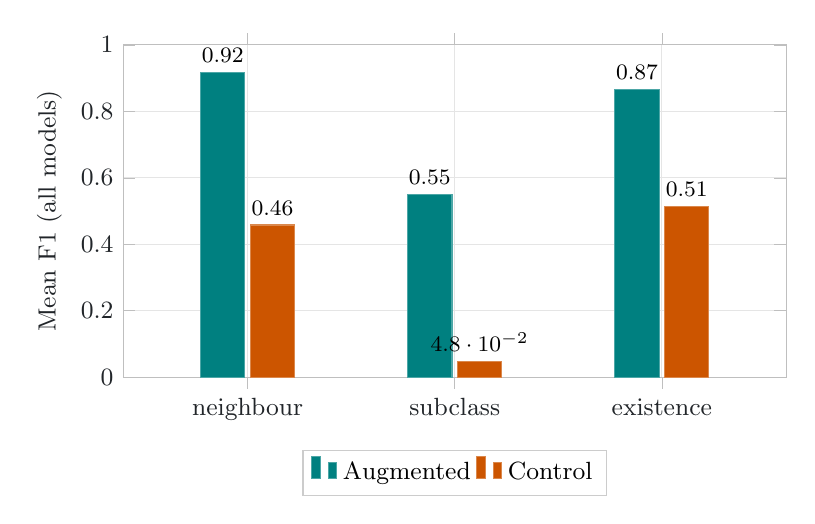
\begin{tikzpicture}
  \begin{axis}[ybar,width=10cm,height=5.8cm,bar width=16pt,ymin=0,ymax=1,ylabel={Mean F1 (all models)},
    symbolic x coords={neighbour,subclass,existence},xtick=data,enlarge x limits=0.3,
    legend style={at={(0.5,-0.22)},anchor=north,legend columns=2,draw=gray!40},
    nodes near coords,nodes near coords style={font=\footnotesize}]
  \addplot[A] coordinates {(neighbour,0.917) (subclass,0.55) (existence,0.865)};
  \addplot[C] coordinates {(neighbour,0.458) (subclass,0.048) (existence,0.513)};
  \legend{Augmented,Control}
  \end{axis}\end{tikzpicture}
  \foot{Biggest gains on proprietary structure (subclasses: +0.50) and niche concepts the base model can't know.}
\end{frame}

\begin{frame}{What it costs}
  \begin{itemize}
    \item Grounding adds context tokens and one retrieval round-trip --- \textbf{optional and per-call}.
    \item Gemini 2.5 Pro: ~4198 prompt tokens/query; GLM-5.2: ~3620 --- modest for the accuracy gained.
    \item \textbf{Budget-bounded \& fail-open:} if the graph is unreachable, the turn proceeds ungrounded --- never blocked.
  \end{itemize}
  \vskip6pt
  {\color{teal0}\textbf{Net:}} a bounded, switchable cost for a large, universal accuracy gain.
  \foot{The binding augments thinking without overpowering the context window.}
\end{frame}

\begin{frame}{The design works}
  \begin{center}
  {\Large A formal ontology, bound pervasively to AI,\\ makes \textbf{every} model more accurate and less hallucinatory.}
  \vskip10pt
  \begin{itemize}
    \item \textbf{+0.44 mean F1} across 5 LLMs; hallucination roughly halved.
    \item Read-pervasive, write-governed, budget-bounded, fail-open --- production-shaped.
    \item One shared brain across tool, consultant and CLI surfaces.
  \end{itemize}
  \vskip12pt
  {\color{burnt}\Large\textbf{VisionFlow}}\;\textbullet\;{\large VisionClaw \textbullet\ Agentbox}\\[4pt]
  {\color{burnt}\large\url{http://www.visionflow.info}}
  \end{center}
\end{frame}

\end{document}
